\newpage
\begin{center}
  \textbf{2 ТЕХНИЧЕСКАЯ РЕАЛИЗАЦИЯ}
\end{center}

\addcontentsline{toc}{section}{2 ТЕХНИЧЕСКАЯ РЕАЛИЗАЦИЯ}

\textbf{2.1 Структура базы данных}
\addcontentsline{toc}{subsection}{2.1 Структура базы данных}

База данных для разрабатываемого приложения состоит из 4 таблиц (рис. 1). Ниже приведено описание каждой таблицы и связей между ними.

\renewcommand{\figurename}{Рисунок}
\begin{figure}[htbp]
    \centering 
    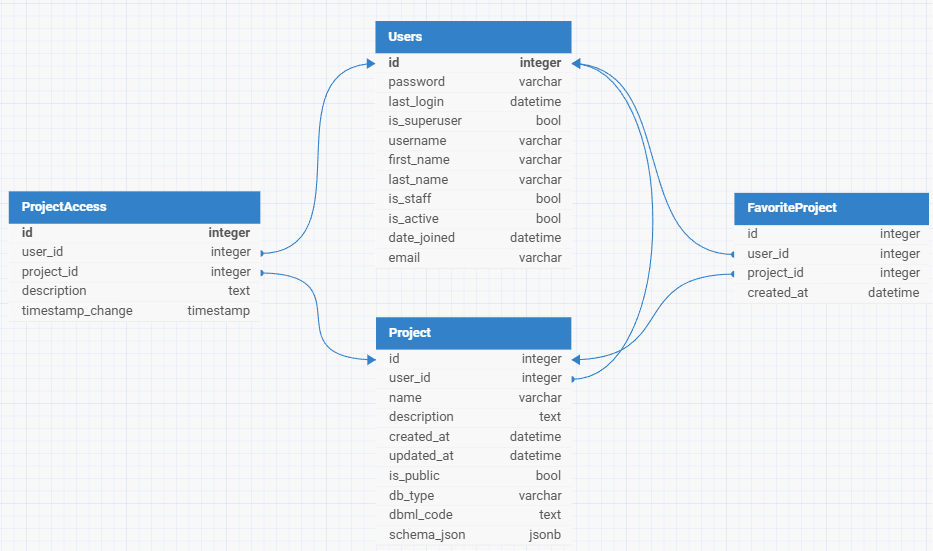
\includegraphics[width=1\textwidth]{db.png} 
    \caption{Структура базы данных}
\end{figure}

Таблица User хранит информацию о зарегистрированных пользователях, их учетные данные и даты регистрации.

• id (integer, primary key, auto increment) – уникальный числовой идентификатор пользователя

• password (varchar(128) not null) – хешированное значение пароля для безопасной аутентификации

• last\_login (datetime null) – метка времени последнего успешного входа в систему

• is\_superuser (boolean not null) – флаг администраторских прав

• username (varchar(150) unique not null) – уникальное имя пользователя, обязательное поле

• first\_name (varchar(150) null) – имя пользователя

• last\_name (varchar(150) null) – фамилия пользователя

• email (varchar(254) unique not null) – электронная почта пользователя, используется для входа

• is\_staff (boolean not null) – флаг доступа к административной панели

• is\_active (boolean not null) – флаг активности учетной записи

• date\_joined (datetime not null) – дата и время регистрации пользователя


Таблица Project содержит данные о созданных пользователями проектах, представляющих собой схемы баз данных.

• id (integer, primary key, auto increment) – уникальный идентификатор проекта

• user\_id (integer not null) – ссылка на владельца проекта

• name (varchar(255) not null) – название проекта с ограничением длины

• description (text null) – описание проекта

• created\_at (datetime not null) – автоматически устанавливаемая дата 
создания

• updated\_at (datetime not null) – автоматически обновляемая дата изменения

• is\_public (boolean default true) – флаг публичной доступности проекта

• db\_type (varchar(20) not null) – тип СУБД (mysql/postgresql/sqlserver/Oracle)

• dbml\_code (text not null) – полное описание схемы в формате DBML

• schema\_json (jsonb not null) – структура проекта в JSON-формате

Таблица FavoriteProject (избранные проекты) - осуществляет связь между пользователями и добавленными в избранное проектами.

• id (integer, primary key, auto increment) – уникальный идентификатор записи

• user\_id (integer not null) – ссылка на пользователя

• project\_id (integer not null) – ссылка на проект

• created\_at (datetime not null) – дата добавления в избранное

Ограничения:
• Уникальный составной индекс (user\_id, project\_id) предотвращает дублирование

• Каскадное удаление при удалении связанных записей

Таблица ProjectAccess (права доступа) - управляет разрешениями пользователей для работы с проектами.

• id (integer, primary key, auto increment) – уникальный идентификатор доступа

• project\_id (integer not null) – ссылка на проект

• user\_id (integer not null) – ссылка на пользователя

• role (varchar(10) not null) – уровень доступа (owner/editor/viewer)

• created\_at (datetime not null) – дата предоставления доступа

Роли доступа:

• owner – полные права владельца

• editor – права на редактирование

• viewer – права только на просмотр

Ограничения:

• Уникальный составной индекс (project\_id, user\_id) для исключения дублирования прав

• Каскадное удаление связанных записей

Связи между таблицами

1. User - Project (один-ко-многим):
Один пользователь (CustomUser) может быть владельцем множества проектов (Project). Связь реализована через поле user\_id в таблице Project, которое ссылается на id в CustomUser. При удалении пользователя все его проекты также удаляются (каскадное удаление).

2. User - FavoriteProject - Project (многие-ко-многим):
Пользователи могут добавлять проекты в избранное. Связь организована через промежуточную таблицу FavoriteProject, где user\_id ссылается на CustomUser, а project\_id - на Project. Уникальный индекс на пару этих полей предотвращает дублирование.

3. User - ProjectAccess - Project (многие-ко-многим):
Система управления доступом к проектам. Таблица ProjectAccess связывает пользователей с проектами через поля user\_id и project\_id, с указанием роли доступа (owner/editor/viewer). Уникальный индекс гарантирует, что каждый пользователь имеет только одну роль в конкретном проекте.

Все связи реализованы с каскадным удалением: при удалении пользователя или проекта автоматически удаляются связанные записи в FavoriteProject и ProjectAccess.


Предложенная структура обеспечивает удобную работу с проектами по моделированию баз данных, включая создание таблиц, полей и связей между ними. 

\

\textbf{2.1.1 Нормализация базы данных}
\addcontentsline{tocdepth}{subsubsection}{2.1.1 Нормализация базы данных}

Таблица User (Пользователи) соответствует третьей нормальной форме (3NF). Первичный ключ id уникально идентифицирует каждого пользователя.
Все атрибуты полностью функционально зависят от первичного ключа. 
Отсутствуют транзитивные зависимости между неключевыми атрибутами. Структура таблицы не содержит повторяющихся групп данных, что соответствует требованиям первой нормальной формы (1NF). Нет частичных зависимостей неключевых атрибутов от первичного ключа, что удовлетворяет второй нормальной форме (2NF).

Таблица Project (Проекты) соответствует третьей нормальной форме. Первичный ключ id однозначно идентифицирует каждый проект. Все атрибуты зависят только от первичного ключа. 
Внешний ключ user\_id корректно связывает проект с владельцем из таблицы CustomUser. Поле schema\_json (тип JSONB) рассматривается как атомарное значение в контексте нормализации. Отсутствуют повторяющиеся группы данных и транзитивные зависимости.

Таблица FavoriteProject (Избранные проекты) соответствует третьей нормальной форме. Составной первичный ключ уникально идентифицирует каждую запись об избранном проекте. Поле created\_at полностью зависит от составного ключа. Внешние ключи user\_id и project\_id поддерживают целостность связей с соответствующими таблицами. Уникальный индекс на пару (user\_id, project\_id) предотвращает дублирование записей. Структура таблицы не содержит избыточных данных или транзитивных зависимостей.

Таблица ProjectAccess (Права доступа) соответствует третьей нормальной форме. Составной первичный ключ (project\_id, user\_id) уникально идентифицирует каждое право доступа. Поля role и created\_at полностью зависят от составного ключа. Внешние ключи project\_id и user\_id обеспечивают ссылочную целостность с таблицами Project и CustomUser соответственно. Система ролей (owner/editor/viewer) реализована без избыточности данных. Отсутствуют транзитивные зависимости между атрибутами.

Все связи между таблицами организованы в соответствии с принципами реляционной модели данных:

1. Связь «один-ко-многим» между CustomUser и Project реализована через внешний ключ user\_id в таблице Project с каскадным удалением, что обеспечивает целостность данных при удалении пользователя.

2. Связь «многие-ко-многим» между пользователями и избранными проектами реализована через промежуточную таблицу FavoriteProject с составным первичным ключом и соответствующими внешними ключами.

3. Связь «многие-ко-многим» между пользователями и проектами с разными уровнями доступа реализована через таблицу ProjectAccess с контролем уникальности сочетания project\_id и user\_id.

Все внешние ключи настроены на каскадное удаление, что поддерживает целостность данных при удалении родительских записей. Отсутствуют циклические зависимости и нарушения реляционных принципов.

\

\textbf{2.2 Алгоритм синхронизации DBML и диаграммы}
\addcontentsline{toc}{subsection}{2.2 Алгоритм синхронизации DBML и диаграммы}

Система поддерживает двустороннюю синхронизацию между DBML-представлением и визуальной диаграммой. Это позволяет пользователям редактировать структуру базы данных как в текстовом формате DBML, так и через визуальный интерфейс, при этом изменения автоматически синхронизируются между обоими представлениями.

\textbf{2.2.1 Структуры данных}
\addcontentsline{tocdepth}{subsubsection}{2.3.1 Структуры данных}

DBML-представление хранится в виде текстового формата (Листинг 1).

Листинг 1 - Структура DBML кода.
\begin{lstlisting}[frame=single]
    Table table_name {
      field_name field_type [constraints]
      ...
    }
    Ref: table1.field > table2.field
\end{lstlisting}

Диаграммное представление структуры базы данных (Листинг 2) храниться в виде словаря, состоящего из узлов, которые представляют каждую таблицу  и содержат следующие обязательные атрибуты:

• key (String) - уникальное название таблицы;

• location (Point) - координаты расположения узла на холсте в пикселях (x, y);

• items (массив) - поля таблицы. Каждое поле содержит в себе id (уникальный идентификатор поля в пределах таблицы), name (название поля), type (тип данных поля), isKey (флаг первичного ключа). 

Каждая связь между узлами описывает отношение между таблицами и содержит в себе информацию о таблицах, между которыми связь, информацию о портах, к которым будет присоединена стрелка связи и категорию, то есть тип связи (Листинг 2). 

Листинг 2 - Структура данных диаграммы.
\begin{lstlisting}[label=some-code,frame=single]
const nodeDataArray = [
    {
        key: "User",
        location: new go.Point(200, 0),
        items: [
            {
                id: 1, name: "id", iskey: true,
                type: "integer"
            },
            { id: 2, name: "name", type: "varchar(255)" }
        ]
    },
    {
        key: 'Project',
        location: new go.Point(500, 0),
        items: [
            {
                id: 1, name: 'id', iskey: true,
                type: "integer"
            },
            { id: 2, name: 'name', type: "varchar(255)" },
        ]
    }
];

const linkDataArray = [
    {
        from: 'User',
        to: 'Project',
        fromPort: 'right_1',
        toPort: 'left_1',
        category: "many-to-one"
    },
];
\end{lstlisting}
